\subsection{Data Gatherer}\label{sec:impl-data-gatherer}
The data gatherer tool has been split into a number of files for readability and maintenance. Additionally, a significant portion of the code written has been tested with automated tests to ensure the quality of the solution. Project structure is initially split between source code and test code folders, named \texttt{src} and \texttt{test} respectively. In each, a number of resource files have been defined to support the program execution, mock server responses, and data or provide additional information.

\begin{figure}[!h]
    \centering
    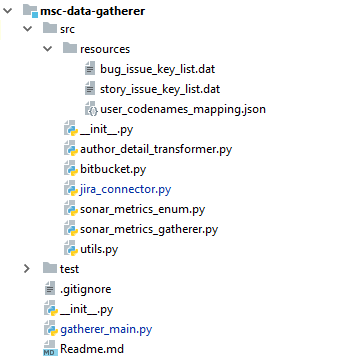
\includegraphics{Figures/impl_src_folder_files.png}
    \caption{Source Files Structure}
    \label{fig:impl-data-gatherer-source-files}
\end{figure}

The source folder structure has been illustrated in Figure \ref{fig:impl-data-gatherer-source-files} and it is comprised of the following elements:
\begin{enumerate}
    \item \texttt{gatherer\_main.py} - included in full in code excerpt \ref{code:gatherer_main.py}. Coordinates all data gathering operations. 
    \item\label{lst:impl.item:jira} \texttt{jira\_connector.py} - Handles all communication and authentication with a given JIRA server.
    \item\label{lst:impl.item:bitbucket} \texttt{bitbucket.py} - handles all communication and authentication with a given Bitbucket server.
    \item\label{lst:impl.item:sonar-metrics-gatherer} \texttt{sonar\_metrics\_gatherer.py} - is responsible for all communication via REST API with Sonar server instance.
    \item\label{lst:impl.item:author-encoder} \texttt{author\_detail\_transformer.py} is responsible for encoding authors' full names into code names to obfuscate sensitive identity details. 
\end{enumerate}

\subsubsection{Main Gatherer}\label{sec:source-code:main-gatherer}

\subsubsection{JIRA Connector}\label{sec:source-code:jira}
The very first operation that the JIRA connector class is responsible for is obtaining a list of JIRA keys. Typically composed of 3 to 4 letters, a key is an abbreviation uniquely identifying a given JIRA project. JIRA keys are obtained from a pre-compiled lists: the \texttt{bug\_issue\_key\_list.dat} and \texttt{story\_issue\_key\_list.dat} files, where the former contains only keys to Story-type tickets, while the latter to bug-type tickets. 
All of the communication with JIRA server happens over its publicly available REST API. In order to access it, base URL is required in the form of \mintinline{html}{<server_name>/jira/rest}.

The JIRA connector then interrogates the server by executing \mintinline{html}{/api/2/issue/{jira_key}} in order to obtain an ID attribute for each ticket. Ticket ID is a necessary parameter required in order to obtain the list of files committed under each ticket.

In the next step, a list of commits for a given JIRA ID is obtained for all code repositories from the \mintinline{html}{/dev-status/1.0/issue/detail?issueId={jira_id}&applicationType=stash} URL. The server response is in JSON format and as Figure \ref{fig:source-code:jira:commit-response} illustrates it is possible for any given commit to include multiple files, per repository. Additionally, many commits can be made under the same ticket, under many repositories. Based on Figure \ref{fig:source-code:jira:commit-response}, it should be assumed that the all of the next steps are executed for all files, under any commit in any repository provided by the above REST call.
\begin{figure}[!h]
    \centering
    \caption{Sample Response from JIRA detailing all commits made under given ticket}
    \label{fig:source-code:jira:commit-response}
    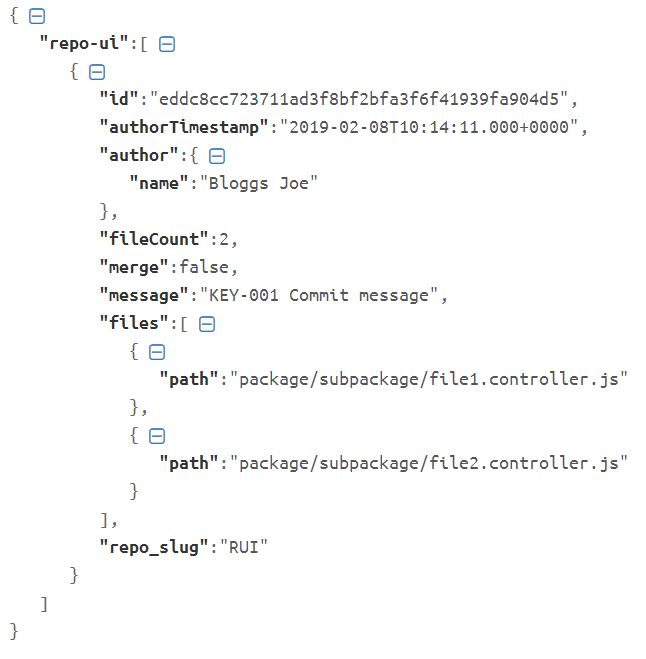
\includegraphics[scale=0.7]{Figures/gatherer/jira_connector_getting_commit_files_response.PNG}
    \caption{Caption}
    \label{fig:my_label}
\end{figure}
    
At this step, a number of infrastructure repositories that are maintenance-only, or ones that are written in languages not supported by Sonar server, thus making it impossible to obtain code quality metrics, have been removed. The repository names to be excluded are matched by a regular expression, from a list of static names compiled based on the domain knowledge of the infrastructure present at the business site. The repositories in question were mainly related to testing framework setup and maintenance, deployment pipelines for specific products and applications present at the business site or automated tests, etc. The list is not provided as it includes product names and it has been considered sensitive by the business owners.
    
In the next step, all merge commits are being removed from the analysis as it would otherwise create duplicate data points. For detailed explanation refer to Section \ref{sec:design}. 

Subsequently, a number of files are removed from the analysis - for listing of what file patterns were ignored, refer to Table \ref{tbl:file-extensions-excluded-from-analysis}. The files were excluded by name and/or extension pattern using regular expression and they represented a number of different categories detailed below. 

Firstly, "Test Files" column included the actual test classes housing the automated test scripts, their corresponding fixtures and object factories and any test configuration required by a given project.

The "Build and Infrastructure" column describes any files required, utilized or produced as part of a given project's build and publishing lifecycle. It also included any files relating to the infrastructure as code, which is heavily utilized in the applications under analysis to codify setup of any given deployment.

The third column, "Interfaces, Enums and Transfer Objects", details patterns for specific source code file for which code coverage doesn't exists as they're not strictly executable. This includes Java or Kotlin interface files, which as they do not have a specific file name associated with them, had to be compiled by trial and error and from own domain knowledge. Additionally, all of the enumerations in Java and Kotlin languages were excluded by utilizing the commonly applied "Enum" suffix. Furthermore, all data transfer object, which in the context of applications under analysis would only contain mutator methods, were excluded by utilizing the "Dto" suffix. 

The "Project Configuration" column refers to any configuration files contained in the project, which can refer to both application object setup, in the form of for example Spring Framework's Beans, as well as build tool files and properties. 
The "Other" column contains all of the files that did not fit any of the above categories. It represents the readme files, database scripts and other setup files.

To reiterate, all of the file patterns included in Table \ref{tbl:file-extensions-excluded-from-analysis} represent files for which no source code metrics could presently, be obtained from Sonar server. Therefore, they were removed to prevent generating noise in the analysis.


    
In the next and final step a list of initial metrics identifying a given commit is compiled. Alongside it, a map containing \texttt{issue\_key}, \texttt{source\_repository}, \texttt{commitId}, \texttt{path} and \texttt{repo\_code}, which is a unique 3-4 character abbreviation identifying a repository, is composed. Complete map containing both commit details as well as information necessary in the subsequent step is returned back to the coordinator file. 
    
For code listing for this step refer to code excerpt \ref{code:jira-connector.py}

\subsubsection{Bitbucket Connector}\label{sec:source-code:bitbucket}
Given data provided by JIRA server from above item interrogates a specified Bitbucket server over REST API in order to obtain details of the previous commit such as author and timestamp. As previously described in Section \ref{sec:design}, List \ref{lst:design:info-from-bitbucket} those details will be used in subsequent analysis steps to provide an indication of developers' level of experience based on seniority as well as familiarity with a given product based on the amount of time spent on the project.
    
Once all those details have been obtained and compiled they are returned to the coordinator file.
Complete code listing is available from code excerpt \ref{code:bitbucket.py}.
 
\subsubsection{Sonar Metrics Gatherer}\label{sec:source-code:sonar-metrics}
Using data gathered by JIRA and Bitbucket steps above it contacts Sonar server for each and every file, for each and every commit under each JIRA ticket and retrieves a specified list of code quality metrics. The list is defined in \texttt{sonar\_metrics\_enum.py} and it is comprehensive. 
    
In order to retrieve code quality metrics first, the expected parameters need to be generated from data retrieved from both JIRA and Bitbucket - the expected data is called project component and it is a unique identifier on Sonar Server for each file ever analyzed. The project component is in a different format for some projects, therefore, it was necessary to model a number of generation use cases, as outlined in the \texttt{sonar\_component\_name\_generator} method in \ref{code:sonar-gatherer.py} code listing.
    
One thing of note is that for different source code languages different metrics, especially with regards to the code coverage metrics can be provided by Sonar. For example, for JavaScript-based languages such as Angular JS there is a separate position for integration, or IT, coverage, whereas for Java and other JVM based languages that metric is rarely provided. In JVM based languages it has been folded into the \texttt{overall code coverage} metric instead.


\subsubsection{Author Detail Transformer}\label{sec:source-code:author-encoder}
it is invoked after code quality metrics have been gathered by \texttt{SonarMetricsGatherer} class.

\subsubsection{Other Utilities}


\begin{table}[h!]
\centering
\caption{Files excluded from the analysis by extension or suffix}
\label{tbl:file-extensions-excluded-from-analysis}
% \begin{tabular}{@{}llll@{}}
% \toprule
% \multicolumn{4}{c}{Exclusion Patterns} \\ \midrule
% .*Test.*.java & .*Interface.*\textbackslash{}.java & .*NameToIndex\textbackslash{}.java & .*\textbackslash{}.jar \\
% .*Test.*.kt & .*Interface.*\textbackslash{}.kt & .*Config.kt & .*Dto.*kt \\
% .*\textbackslash{}.e2e-spec.js & .*\textbackslash{}.stub.js & .*\textbackslash{}.po.js & .*spec.js \\
% .*\textbackslash{}.ico & .*\textbackslash{}.npmrc & .*\textbackslash{}.conf.js & .*gulpfile.js \\
% .*ColumnDef.js & .*Spec.js & .*Decorator.js & \textbackslash{}.eslintrc \\
% .*\textbackslash{}.gitattributes & .*\textbackslash{}.sql & .*\textbackslash{}.csv & .*\textbackslash{}.xlsx \\
% .*\textbackslash{}.txt & .*\textbackslash{}.xlsm & .*\textbackslash{}.yaml & .*\textbackslash{}.yml \\
% .*WriteService.* & .*DeleteService.* & .*CreateService.* & .*\textbackslash{}.lock \\
% .*.gradle & .*\textbackslash{}.?factory.js & .*\textbackslash{}.css & .*.config.js \\
% .*Config.java & .*\textbackslash{}.html & .*\textbackslash{}.svg & .*ColumnDefs.js \\
% .*\textbackslash{}.gz & .*ReadService.* & \textbackslash{}.gitignore & .*\textbackslash{}.json \\
% .*\textbackslash{}.war & .*Enum.*kt & .*\textbackslash{}.scss & .*factories.js \\
% .*Jenkinsfile.* & .*\textbackslash{}.xml & .*\textbackslash{}.md & .*\textbackslash{}.properties \\ \bottomrule
% \end{tabular}

\begin{tabular}{@{}lllll@{}}
\toprule
Test Files & \begin{tabular}[c]{@{}l@{}}Build and Deployment \\ infrastructure\end{tabular} & \begin{tabular}[c]{@{}l@{}}Interfaces, Enums \\ and Transfer Objects\end{tabular} & Project configuration & Other \\ \midrule
.*Test.*.java & .*\textbackslash{}.war & .*Interface.*\textbackslash{}.java & .*Config.java & .*\textbackslash{}.csv \\
.*Test.*.kt & .*Jenkinsfile.* & .*Interface.*\textbackslash{}.kt & .*Config.kt & .*\textbackslash{}.css \\
.*\textbackslash{}.e2e-spec.js & .*\textbackslash{}.jar & .*ReadService.* & .*.config.js & .*\textbackslash{}.svg \\
.*\textbackslash{}.stub.js & .*\textbackslash{}.npmrc & .*Enum.*kt & .*.gradle & .*\textbackslash{}.scss \\
.*Spec.js & .*\textbackslash{}.yml & .*NameToIndex\textbackslash{}.java & \textbackslash{}.gitignore & .*\textbackslash{}.md \\
.*\textbackslash{}.?factory.js & .*\textbackslash{}.lock & .*CreateService.* & .*\textbackslash{}.gitattributes & .*\textbackslash{}.json \\
.*\textbackslash{}.po.js & .*gulpfile.js & .*WriteService.* & .*\textbackslash{}.properties & .*\textbackslash{}.xlsx \\
.*spec.js & \textbackslash{}.eslintrc & .*DeleteService.* &  & .*\textbackslash{}.ico \\
.*ColumnDefs.js & .*\textbackslash{}.conf.js & .*Dto.*kt &  & .*\textbackslash{}.txt \\
.*factories.js & .*\textbackslash{}.yaml & .*Decorator.js &  & .*\textbackslash{}.gz \\
.*ColumnDef.js &  &  &  & .*\textbackslash{}.sql \\
 &  &  &  & .*\textbackslash{}.xlsm \\
 &  &  &  & .*\textbackslash{}.html \\
 &  &  &  & .*\textbackslash{}.xml \\ \bottomrule
\end{tabular}
\end{table}




\begin{landscape}

\begin{code}
\captionof{listing}{Main data gathering component - the coordinator}
\label{code:gatherer_main.py}
\inputminted{python}{source_code/gatherer.py}
\end{code}

\begin{code}
\captionof{listing}{JIRA Connector - extracts relevant metrics from a given JIRA ticket}
\label{code:jira-connector.py}
% \begin{minted}[breaklines]{python}
\inputminted{python}{source_code/jira_connector.py}
% \end{minted}
\end{code}

\begin{code}
 \captionof{listing}{Bitbucket connector - retrieves commit metrics for a given file}
 \label{code:bitbucket.py}
\inputminted{python}{source_code/bitbucket_connector.py}
 \end{code}
 
 \begin{code}
 \captionof{listing}{Sonar connector - retrieves code quality metrics for a given file}
 \label{code:sonar-gatherer.py}
 
 \inputminted{python}{source_code/SonarMetricsGatherer.py}
 
 \end{code}

\end{landscape}
